\documentclass[10pt, a4paper, hidelinks]{article}
\usepackage[paper=a4paper, left=2cm, right=2cm, bottom=2cm, top=3cm]{geometry} %ajustar m�rgnens
\usepackage[latin1]{inputenc}
\usepackage[spanish]{babel}
\usepackage{caratula}
\usepackage{enumitem} 
\usepackage{hyperref}
\usepackage{mathtools}
\usepackage[font=small,labelfont=bf]{caption}
\newcommand\floor[1]{\lfloor#1\rfloor}
\newcommand\ceil[1]{\lceil#1\rceil}
%\usepackage{clrscode3e} Estilo Cormen
\usepackage[spanish,onelanguage,ruled,vlined,nofillcomment]{algorithm2e}
\usepackage{algpseudocode}
\usepackage{xcolor}
\usepackage[final]{pdfpages} % para agregar el enunciado
%%%%%%%%%%%%%% Formato de p�rrafos %%%%%%%%%%%%%%%%%%
\setlength{\parindent}{2em}
\setlength{\parskip}{3pt}
%%%%%%%%%%%%%%%%%%%%%%%%%%%%%%%%%%%%%%%%%%%%%%%%%%%%%%%
\usepackage{fancyhdr}
\usepackage{lastpage}
\setlength{\intextsep}{0.2cm}
\pagestyle{fancy}
\lhead{Sistemas Operativos}
\rhead{$1^{\mathrm{er}}$ cuatrimestre de 2018}

\LinesNumbered
\DontPrintSemicolon

\newcommand{\comp}[1]{$\mathcal{O}(#1)$}

%%%%%%%%%%%%%%%%%%% Macro para comentar codigo %%%%%%%%%%%%%%%%%%%%%%%%%
\newcommand{\comentario}[1]{
\SetKwComment{Comment}{/* }{ */}
\textcolor{blue}{\Comment*[h]{{#1}}}
}
%%%%%%%%%%%%%%%%%%%%%%%%%%%%%%%%%%%%%%%%%%%%%%%%%%%%%%%%%%%%%%%%%%%%%%%%

\begin{document}

\materia{Sistemas Operativos}
\submateria{Primer cuatrimestre del 2018}
\titulo{Trabajo Pr�ctico 2: \texttt{blockchain}}
\integrante{Budi�o, Gabriel Fabricio}{046/16}{gabriel.f.budi@gmail.com} % obligatorio 
\integrante{Garro, Dami�n Eugenio}{354/16}{damian.garro.mst@gmail.com} % obligatorio 
\integrante{Rozenberg, Uriel Jonathan}{838/12}{rozenberguriel@gmail.com} % obligatorio 

\maketitle

\tableofcontents
\pagenumbering{gobble}

\pagebreak
\pagenumbering{arabic}
\cfoot{\thepage /\pageref{LastPage}}

\section{Introducci�n}
Para este trabajo se deb�a implementar una cadena de bloques ($blockchain$) utilizando la interfaz MPI con el objetivo de desarrollar conocimientos en sistemas distribuidos.

A continuaci�n se presenta un breve resum�n de la resoluci�n de cada ejercicio as� como de la experimentaci�n realizada. El enunciado completo se encuentra en el Ap�ndice A.

\section{Resoluci�n}
\subsection{Ejercicio 1}
La funci�n \texttt{broadcast\_block} es la encargada de comunicar al resto de los nodos que se ha minado un bloque. El pseudoc�digo de la misma es el siguiente:

\begin{algorithm}[H]
\SetKwProg{Fn}{Funci�n}{}{fin}
\SetAlgoLined
\Fn{broadcast\_block(bloque)}{
	\ForEach{nodo n distinto del comunicador}{
		enviar(bloque, n) \\
	}
}
\caption{\texttt{broadcast\_block}}
\end{algorithm}

Para referenciar a un proceso ($nodo$) usamos su \texttt{rank} dentro del communicator global \texttt{MPI\_COMM\_WORLD}. Contamos con las variables \texttt{mpi\_rank} y \texttt{total\_nodes}. As�, para cada \texttt{mpi\_rank} + 1 $\leq i \leq$ \texttt{mpi\_rank} + \texttt{total\_nodes}, definimos $destino$ como $i$ $mod$ \texttt{total\_nodes} y enviamos el mensaje usando \texttt{MPI\_Send} con $destino$, $bloque$ y el tag \texttt{TAG\_NEW\_BLOCK} como par�metros.
 
\subsection{Ejercicio 2}

\subsection{Ejercicio 3}

\subsection{Ejercicio 4}

\subsection{Ejercicio 5
}
\section{Experimentaci�n}


\newpage
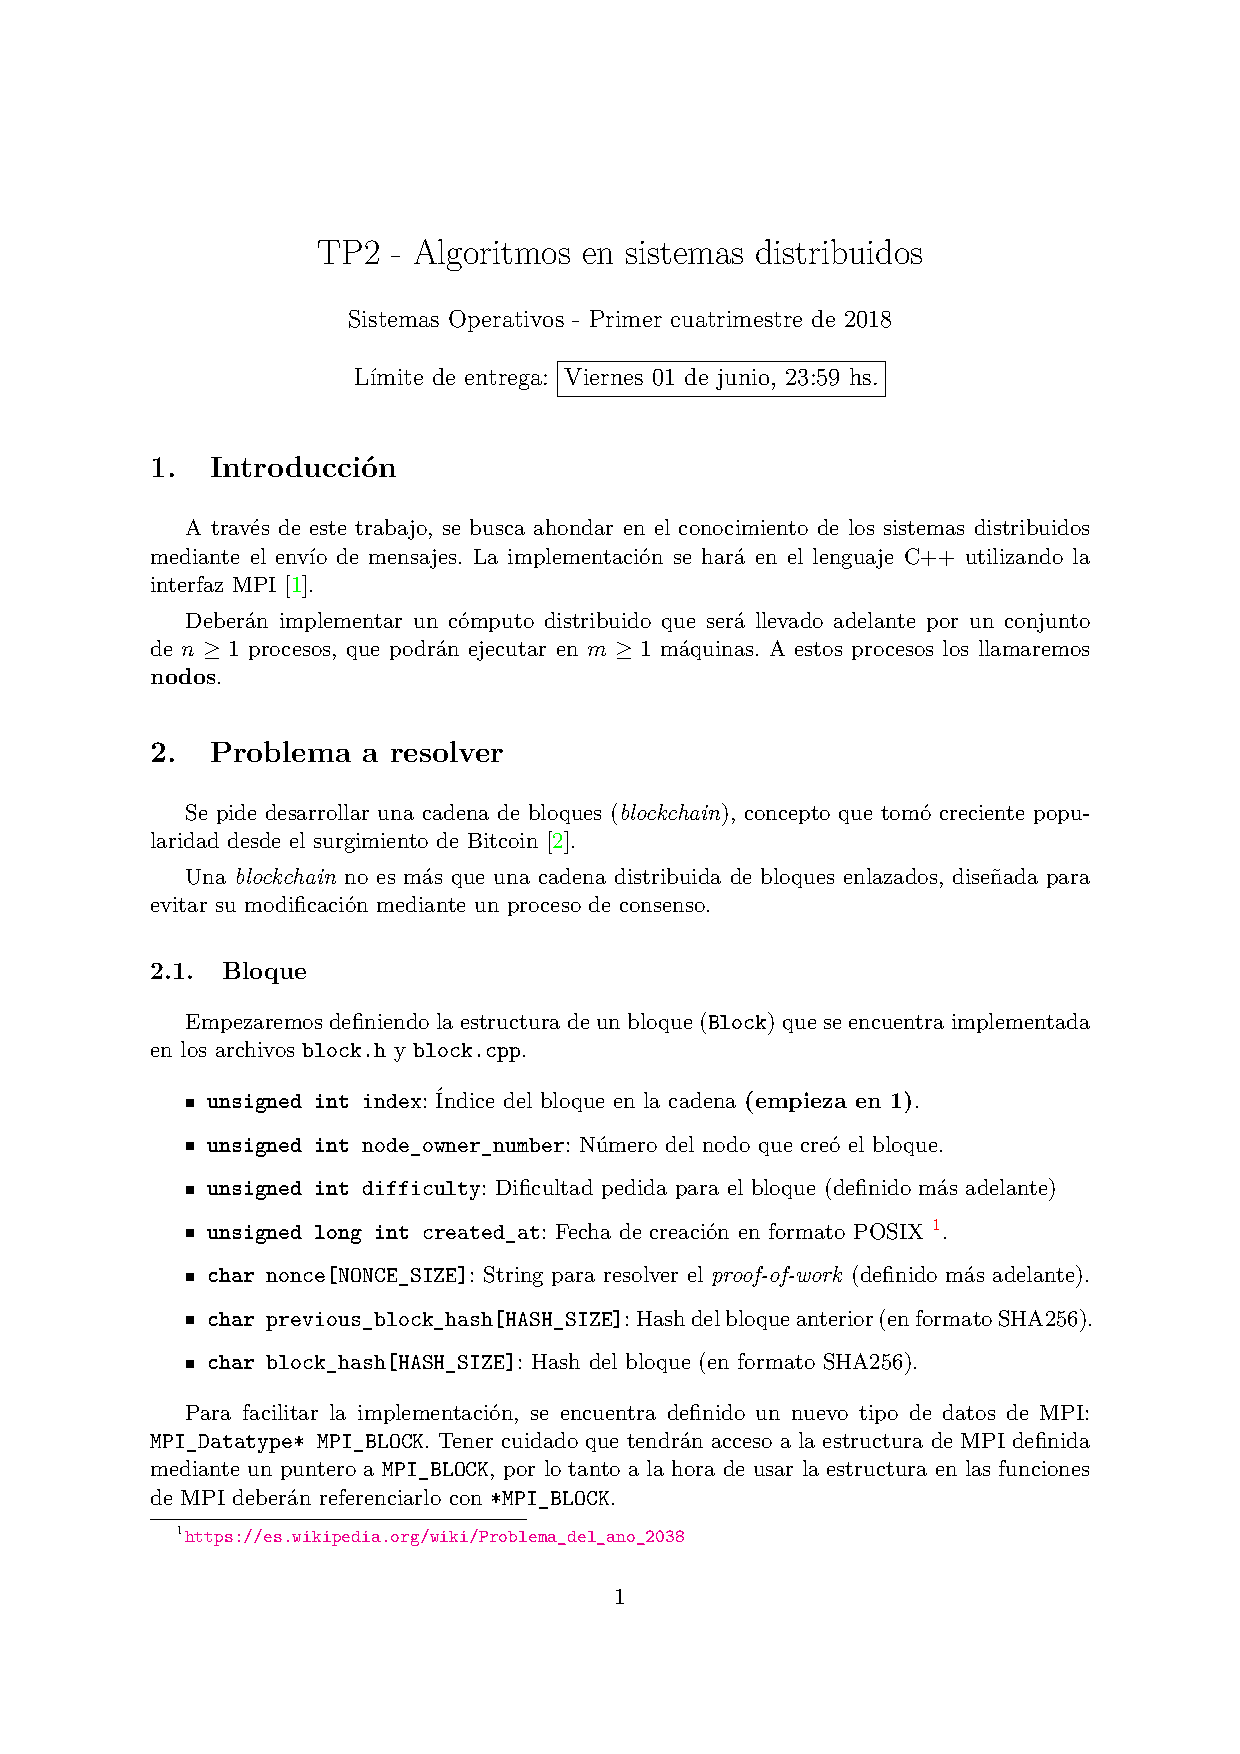
\includepdf[scale=0.75,pages=1,pagecommand=\section{Ap�ndices}
\subsection{Ap�ndice A - Enunciado}]{../enunciado.pdf}
\includepdf[scale=0.75,pages=2-,pagecommand=]{../enunciado.pdf}

\subsection{Ap�ndice B - Aclaraciones}

\end{document}

